%!TEX root = farm.tex


\section{Evaluation}\label{sec:evaluation}
The evaluation compare the performance of the NVIDIA's standard firmware and we developed firmware used FARM.
Table \ref{tab:environment} shows the evaluation environment.
This evaluation measure the overhead of measuring the execution time in the NVIDIA's firmware and the we developed firmware on Gdev\cite{kato:gdev}\cite{kato:gdev2} of GPGPU runtime and resource management engine set.
This execution time is the time to copy of the data into device, the process execution, 
the copy of the data into host.
\par
Measurement results were concentrated in the following over 7msec and less 2msec.
This phenomenon occurred both firmware.
That because GPU's program are many things influence compared to the CPU Program.
Specifically, these are device memory, device driver, GPU cache and GPU memory.
Thus we divide over 7 msec are ``case A'', and less 2 msec are ``case B''.
We compare the average each case A and case B.
Figure \ref{fig:goodcase} shows result of case A.
Also figure \ref{fig:badcase} shows result of case B.
The abscissa axis is Sample program name.
The vertical axis is Execution time (msec).
The blue is the NVIDIA's standard firmware, also the red is the we developed firmware.
Figure \ref{fig:goodcase}, \ref{fig:badcase} can be as seen almost no overheads. 
It is the largest overhead, the case A is 0.003msec of madd, it was 2.31\%.
also it was the lowest overhead, the case B is -0,002msec, it was -1.74\%.
In this way, result has been increased execution time and decreased execution time.
Thus, it is within the range of error at execution time from a range of numbers that was measured is wide.
In addition, if you want to use the GPU application, there will be less affected because the processor core for processing time increases.
For example, The total time of madd in NVIDIA'S standard firmware is 21.842msec, this total time is between finished program from the start program by host.
The execution time overhead occupy relatively small 0.01\% of the total time
Thus, the overhead of firmware developed by our development environment is within the allowable range.
It follows from what has been said that developing firmware by this our development environment is a valid one.
\par
The total time includes the time required to generate GPU context, Memory allocation and Memory release time. 
madd by the running NVIDIA's standard firmware
The total time is 214 msec at the madd first execution times by the NVIDIA standard firmware.
The second total time is 20 msec, this result is a big gap to the first execution time.
Further, the our developing firmware get the same results to NVIDIA standard firmware.
Because the firmware generate the GPU context when the first run, and then, the firmware secondly running use GPU context generated by the first run.
Thus, it takes a long time to generate the GPU context.
This problem findings obtained by firmware development and evaluate.

\begin{table}[!t]
 \caption{Evaluate Environment} 
 \label{tab:environment}
 \hbox to\hsize{\hfil
 \begin{tabular}{|l|l|}\hline
  CPU &  Intel core i7 2600 \\\hline
  GPU &  NVIDIA GeForce GTX480 \\\hline
  Memory & 8GB \\\hline
  Kernel & Linux 2.6.42.12-1.fc15.x86\_64 \\\hline
  Device driver & PSCNV \\\hline
 \end{tabular}\hfil}
\end{table}

\begin{figure}
\begin{center}
\hfil
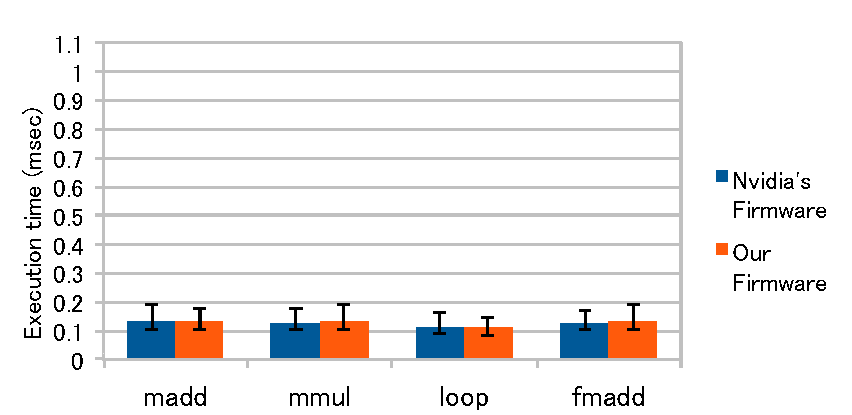
\includegraphics[width=8cm]{./img/good_case.pdf}
\end{center}
\caption{Execution Time of Gdev Sample Program : Case A}
\label{fig:goodcase}
\end{figure}

\begin{figure}
\begin{center}
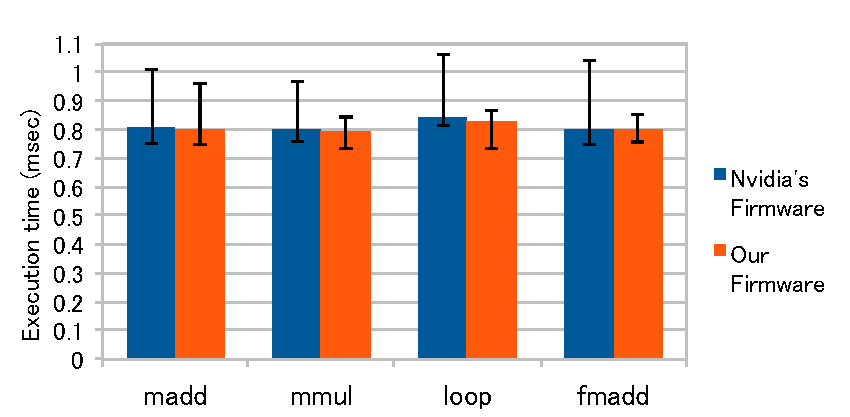
\includegraphics[width=8cm]{./img/bad_case.pdf}
\end{center}
\caption{Execution Time of Gdev Sample Program : Case B}
\label{fig:badcase}
\end{figure}


